\documentclass[9pt, xcolor=table]{beamer}

\usepackage[utf8]{inputenc}
\usepackage[round, comma]{natbib}
\usepackage{amsmath}
\usepackage{hyperref}
\usepackage{amsfonts}
\usepackage{verbatim}
\DeclareMathOperator*{\argmin}{arg\,min}



\mode<presentation> {

\usetheme{Madrid}

\setbeamertemplate{navigation symbols}{} 
\useinnertheme{circles}
\definecolor{greenish}{RGB}{0, 153, 76}
\usecolortheme[named=greenish]{structure}
}

\setbeamertemplate{headline}
{%
  \begin{beamercolorbox}[ht=3.5ex,dp=1.125ex,%
      leftskip=.3cm,rightskip=.3cm plus1fil]{section in head/foot}
    \usebeamerfont{section in head/foot}\usebeamercolor[fg]{section in head/foot}%
\insertsectionnavigationhorizontal{\paperwidth}{\hskip0pt plus1fill}{\hskip0pt plus1fill}
  \end{beamercolorbox}%
  \begin{beamercolorbox}[colsep=1.5pt]{middle separation line head}
  \end{beamercolorbox}
  \begin{beamercolorbox}[colsep=1.5pt]{lower separation line head}
  \end{beamercolorbox}
}

\title[Interpretation of black box models]{Interpretation of black box models using tree-based surrogate models \newline \small{Simulations}}
\author[Sofia Loibl]{Sofia Loibl}
\institute[LMU]{LMU München}
\date{\today}

\begin{document}

\begin{frame}
\titlepage 
\end{frame}


\begin{frame}
\frametitle{Outline} 
\tableofcontents 
\end{frame}

\section{Selection Bias}
\begin{frame}{Selection Bias}
\textbf{Goal:} 

Comparison of SLIM, MOB and CTree with respect to selection bias
\vspace{0.5cm}


\textbf{Selection bias:} 

An algorithm for recursive partitionig is called unbiased when, under the conditions of the null hypothesis of independence between a response $Y$ an covariates $X_{1},...X_{m}$ the probability of selecting covariate $X_{j}$ is $1/m$ for all $j = 1,...,m$ regardless of the measurement scales of number of missing values. \citep{Hothorn.2006}

\end{frame}

\begin{frame}{Selection Bias}

\textbf{Scenario 1 Data:}  $1000$ simulation runs with $n= 100$
\begin{itemize}
    \item $X_{1}, X_{2} \sim U(0,1) $
    \item $X_{3} \sim U(0,1)$ and rounded to one digit
    \item $X_{4}$ binary
    \item $X_{5}$ categorical with 5 levels
    \item $X_{6}$ categorical with 8 levels
    \item $Y \sim N(0,1)$

\end{itemize}

\end{frame}
\begin{frame}{Selection Bias}
\begin{table}
\caption{Relative frequency of selecting covariate $X_i$ as splitting variable}

\centering
\begin{tabular}[t]{l|l|r|r|r|r|r|r}
\hline
  & & SLIM & SLIM Anova & SLIM R2 & SLIM R2 adj & MOB & CTree\\
\hline
x1 & U(0,1) & 44.1 & 19.1 & 0 & 14.9 & 27.2 & 26.1\\
x2 & U(0,1) & 39.2 & 17.7 & 0 & 13.8 & 23.8 & 24.4\\
x3 & U(0,1) rounded 1 & 11.9 & 19.3 & 0 & 14.5 & 27.2 & 28.4\\
x4 & binary & 1.3 & 17.2 & 0 & 13.9 & 20.6 & 20.4\\
x5 & 5 categories & 2.1 & 14.2 & 9.7 & 20.4 & 1.2 & 0.7\\
x6 & 8 categories & 1.4 & 12.5 & 90.3 & 22.5 & 0 & 0\\
\hline
\end{tabular}
\end{table}
\end{frame}

\begin{frame}{Performance Comparison}


\textbf{Procedure:} 

For each simulation run (500 repetitions)
\begin{enumerate}
    \item create simulation data and perform train/test split (2/3)
    \item fit black box model to the training data and measure training and generalization performance ($R^2$ and MSE)
    \item For each model in SLIM, MOB, CTree fit surrogate model to the original training data to measure accuracy (training and generalization) and to the blackbox output to measure fidelity (training and generalization)
\end{enumerate}

\textbf{Note:} All three Methods are forced to generate models with the same terminal node size, i.e. no pruning except fixed tree depth and minimum node size is used

\end{frame}

\section{Performance}
\begin{frame}{Performance Comparison}
\textbf{Question:} 
\textbf{simulation scenarios:}
\begin{enumerate}
    \item \textbf{Linear smooth} $n= 1500$ $$ Y = X_1 + 4 \cdot X_2 + 3 \cdot X_2 \cdot X_3 + 5\cdot X_2\cdot X_4 + X_5 + \epsilon $$
    $X_1,..., X_5 \sim U(-1,1)$, $X_6, X_7 \sim N(0,1)$, $\epsilon \sim N(0, sd_{data})$
    
    \item \textbf{Linear Categorical} $n= 1500$ $$ Y =  0.5\cdot X_{1} - 8\cdot X_2 + 16\cdot X_2\cdot \mathbf{I}_{X_3 = 0} + 8\cdot X_2\cdot \mathbf{I}_{mean(X_1 > X_1)} + \epsilon $$
    $X_1, X_2 \sim U(-1,1)$, $X_3, ..., X_5 \sim Bern(0.5)$, $X_6 \sim N(0,1)$,  $\epsilon \sim N(0, sd_{data})$
    
    \item \textbf{Linear Mixed}  $n= 3000$
    \begin{align*}
    Y = & 4 \cdot X_2 + 2 \cdot X_4 + 2 \cdot X_6 + 2 \cdot X_8 + 4 \cdot X_2 \cdot X_1 + 8 \cdot X_2 \cdot \mathbf{I}_{X_3 = 0} + 10 \cdot X_2 \cdot X_6  \cdot \mathbf{I}_{X_5 = 1} \\
    & + 8 \cdot X_2 \cdot X_7 + 3 \cdot X_1 \cdot X_3 + 3 \cdot X_8 \cdot X_10 + 3 \cdot X_7 \cdot X_9     
    \end{align*}
    $X_1, X_2 \sim U(-1,1)$, $X_3, ..., X_5 \sim Bern(0.5)$, $X_6, ... X_20 \sim N(0,1)$,  $\epsilon \sim N(0, sd_{data})$
\end{enumerate}
    
\end{frame}

\begin{frame}{Performance Comparison}
\begin{figure}
    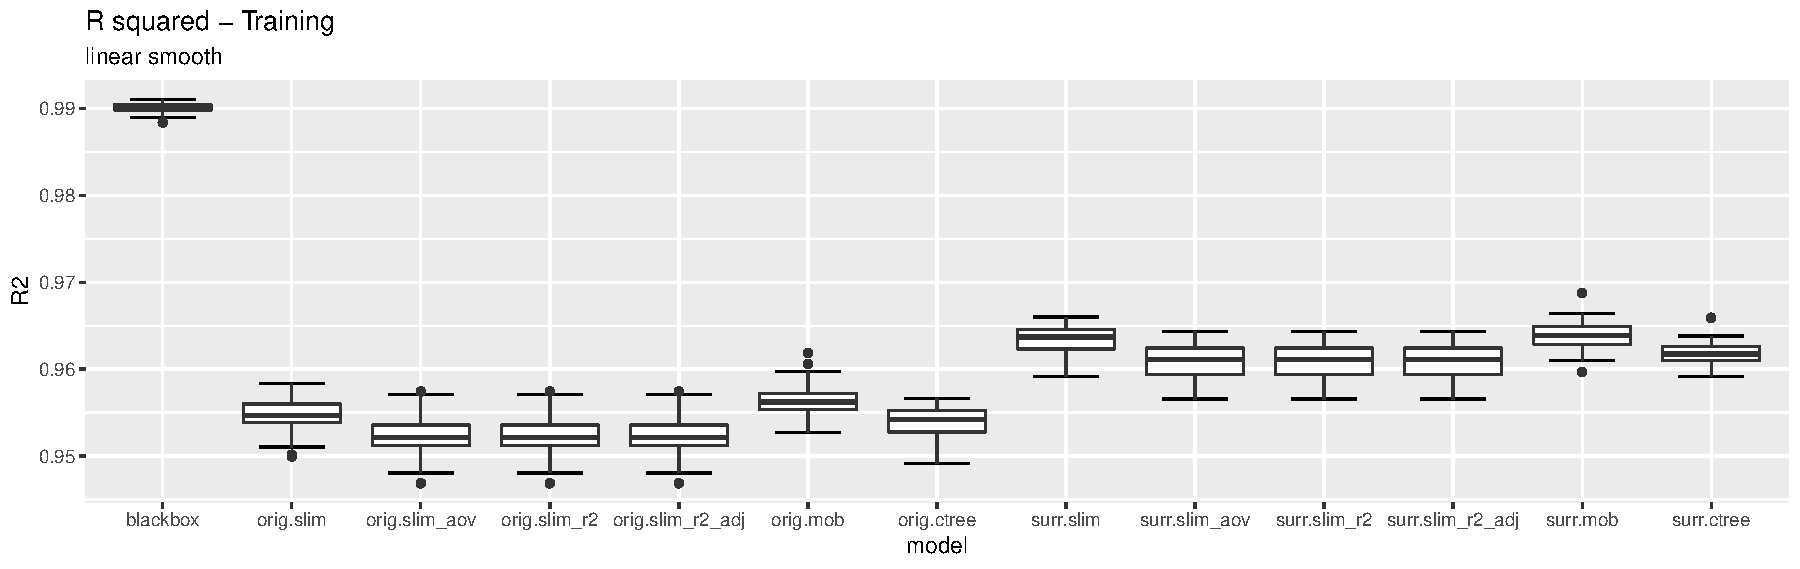
\includegraphics[width=11cm]{Figures/Performance/linear_smooth/r2_train.pdf}
\end{figure}
\end{frame}

\begin{frame}{Performance Comparison}
\begin{figure}
    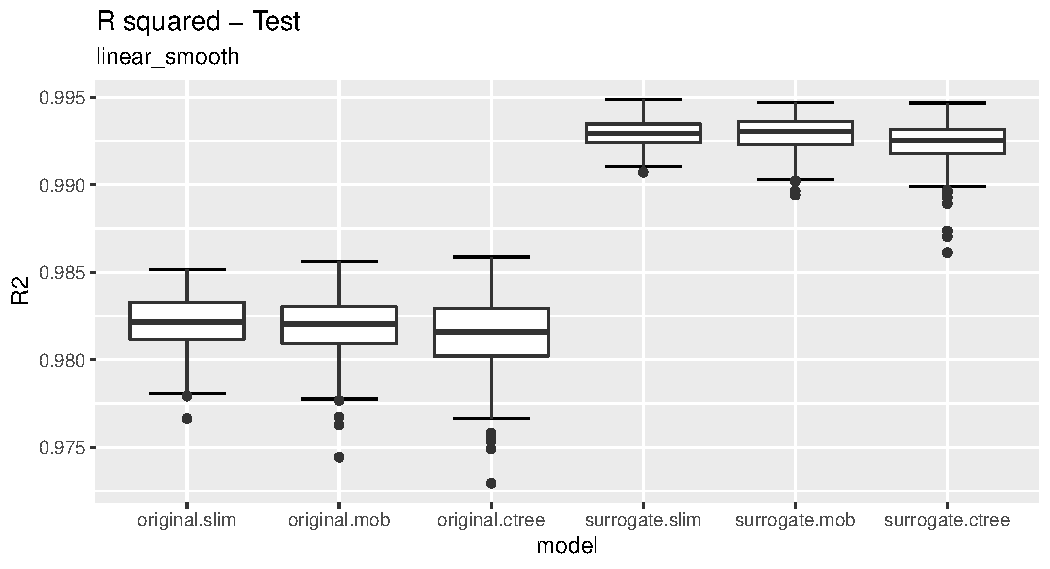
\includegraphics[width=11cm]{Figures/Performance/linear_smooth/r2_test.pdf}
\end{figure}
\end{frame}

\begin{frame}{Performance Comparison}
\begin{figure}
    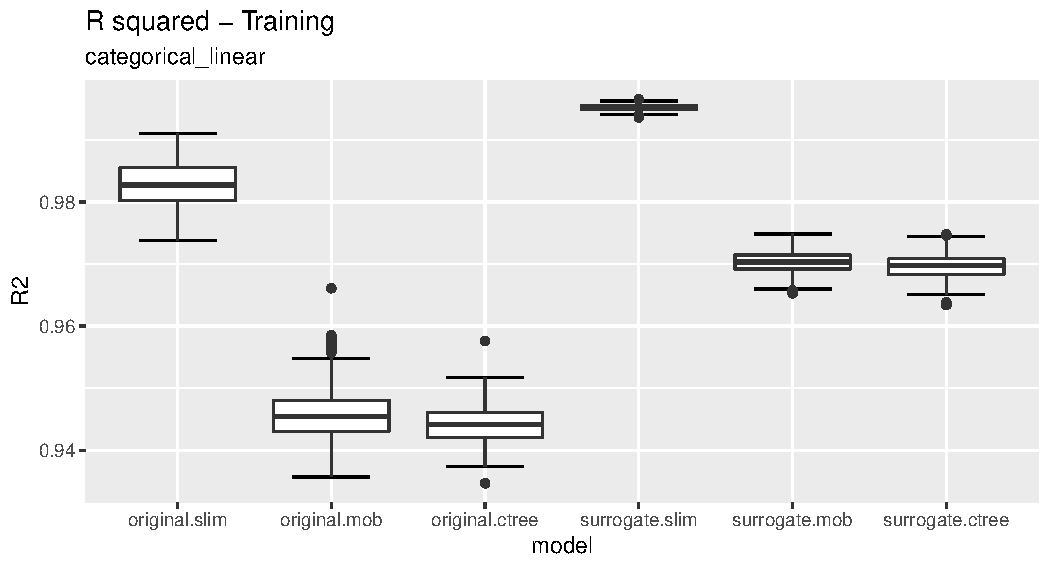
\includegraphics[width=11cm]{Figures/Performance/categorical_linear/r2_train.pdf}
\end{figure}
\end{frame}

\begin{frame}{Performance Comparison}
\begin{figure}
    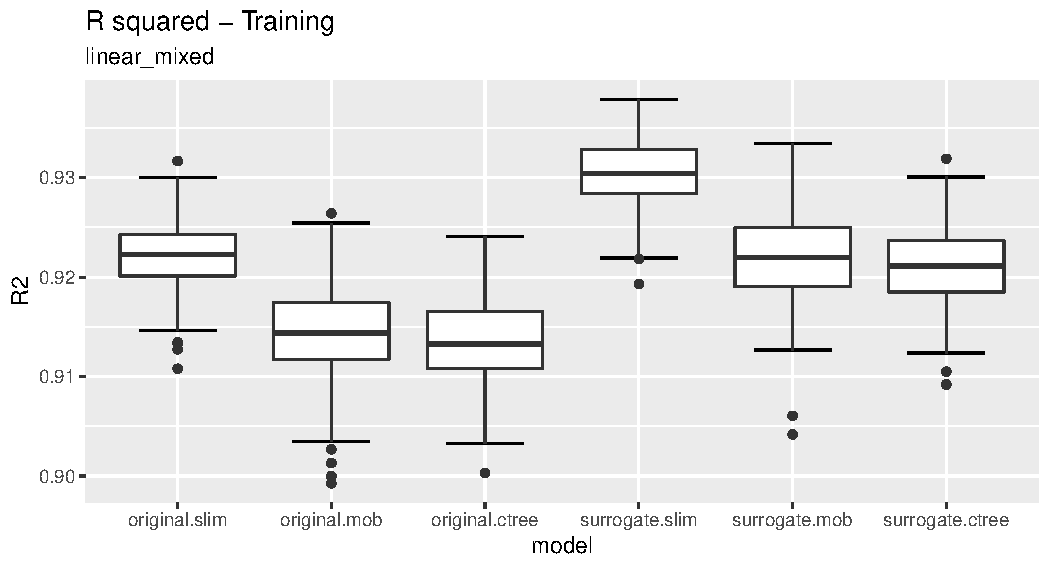
\includegraphics[width=11cm]{Figures/Performance/linear_mixed/r2_train.pdf}
\end{figure}
\end{frame}


\section{Stability}
\begin{frame}{Stability Comparison}
\textbf{Procedure:} 
\begin{enumerate}
    \item create simulation data and train black box model on the data (this dataset is only used to train the black box model)
    \item for each simulation run 
    \begin{enumerate}
        \item create a new dataset and perform train/test split
        \item calculate blackbox predictions for the new dataset
        \item For each model in SLIM, MOB, CTree fit surrogate model to the new training dataset to measure accuracy (training and generalization) and to the new training data and the predicted blackbox output to measure fidelity (training and generalization)
        \item count number of terminal nodes in for the surrogate model and the tree based model on the original 
    \end{enumerate}
\end{enumerate}
\end{frame}

\begin{frame}{Stability Comparison}
\begin{figure}
    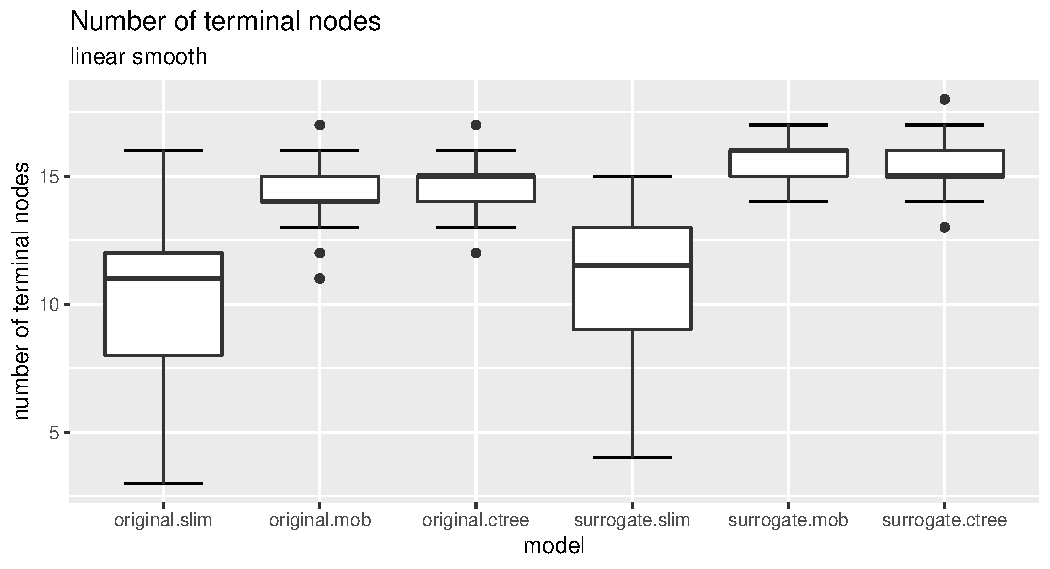
\includegraphics[width=11cm]{Figures/Stability/linear_smooth/nofnodes.pdf}
\end{figure}
\end{frame}


\begin{frame}{Stability Comparison}
\begin{figure}
    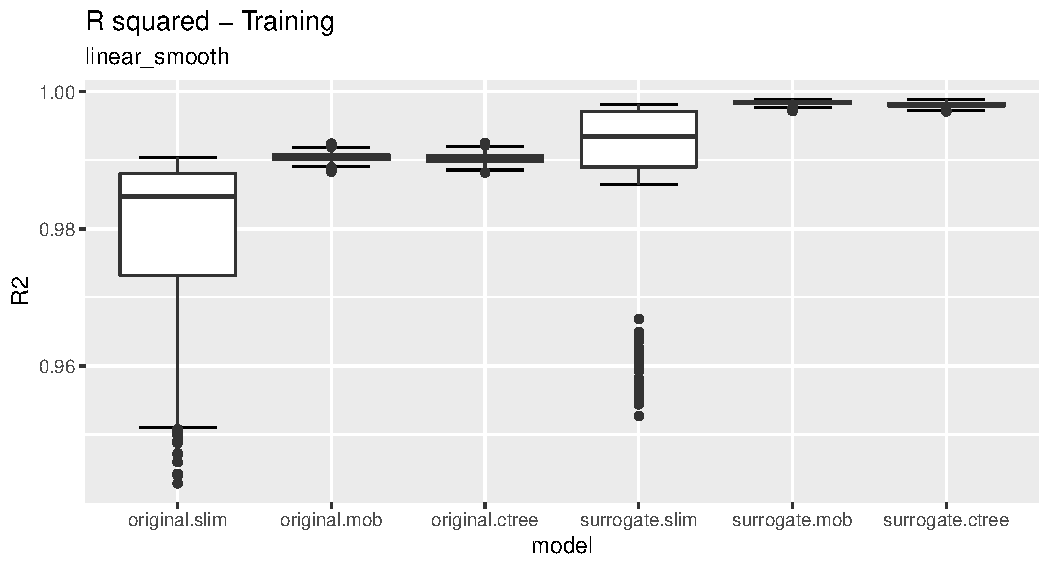
\includegraphics[width=11cm]{Figures/Stability/linear_smooth/r2_train.pdf}
\end{figure}
\end{frame}

\begin{frame}{Stability Comparison}
\begin{figure}
    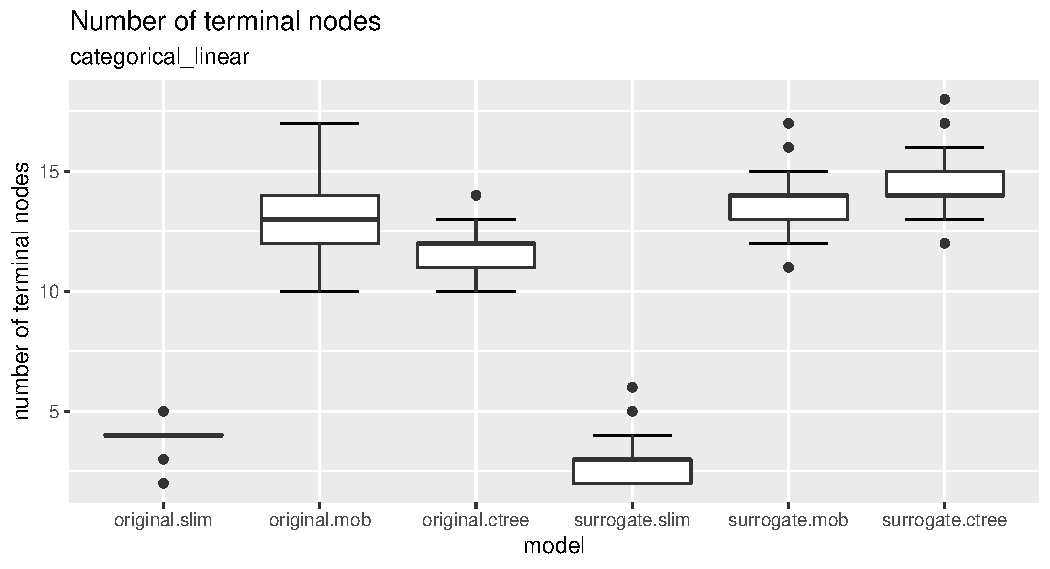
\includegraphics[width=11cm]{Figures/Stability/categorical_linear/nofnodes.pdf}
\end{figure}
\end{frame}

\begin{frame}{Stability Comparison}
\begin{figure}
    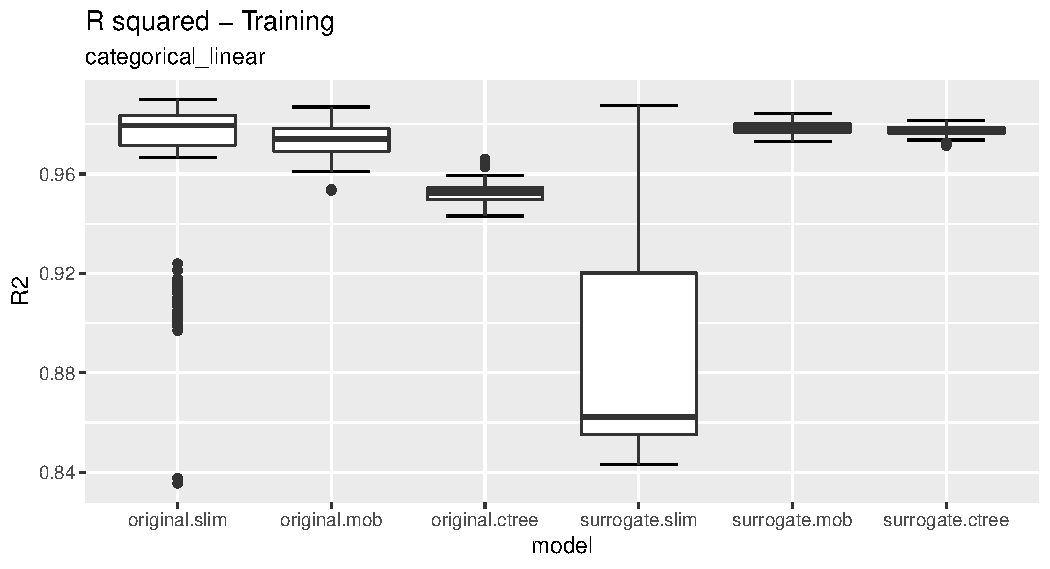
\includegraphics[width=11cm]{Figures/Stability/categorical_linear/r2_train.pdf}
\end{figure}
\end{frame}

\begin{frame}{Stability Comparison}
\begin{figure}
    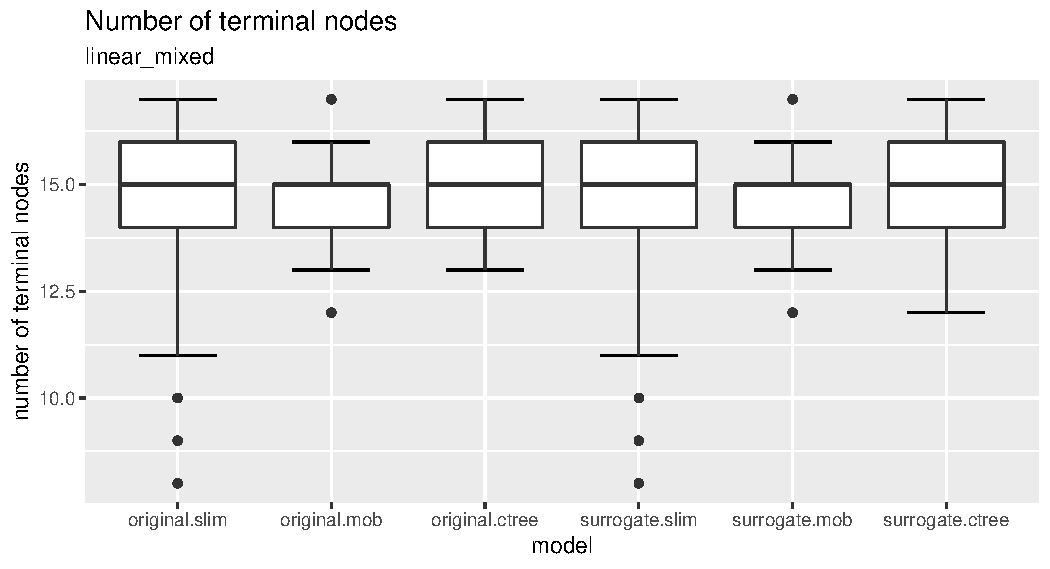
\includegraphics[width=11cm]{Figures/Stability/linear_mixed/nofnodes.pdf}
\end{figure}
\end{frame}

\begin{frame}{Stability Comparison}
\begin{figure}
    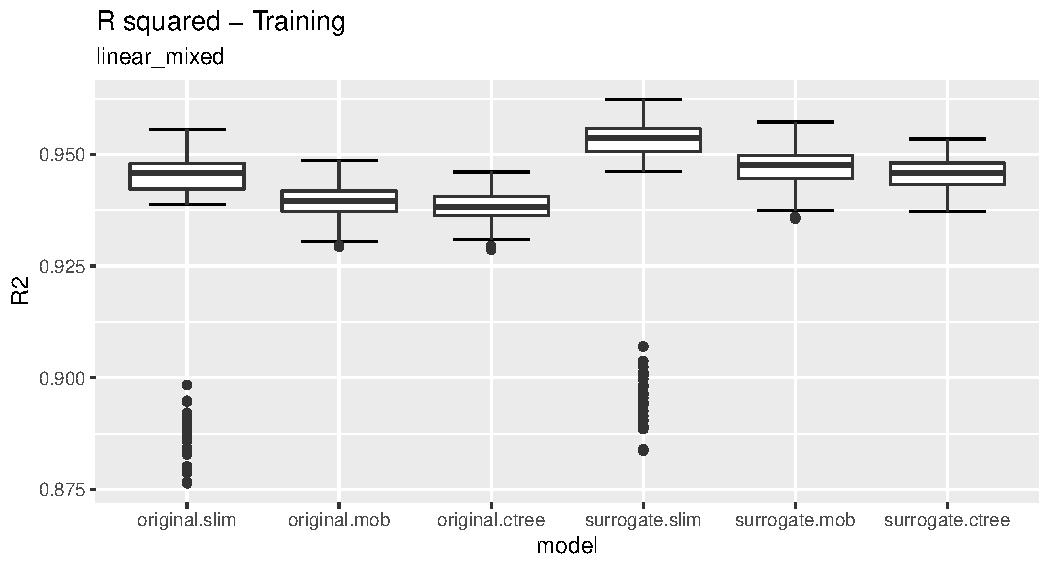
\includegraphics[width=11cm]{Figures/Stability/linear_mixed/r2_train.pdf}
\end{figure}
\end{frame}


\begin{frame}{Bibliography}
    \bibliography{bibliography}
    \bibliographystyle{dcu}

\end{frame}
\end{document}